\documentclass[
aps,
prx,
showpacs,
preprintnumbers,
twocolumn,
superscriptaddress,
10pt,
]{revtex4-2}

\bibliographystyle{apsrev4-2}

% Fonts
\usepackage[T1]{fontenc}
\usepackage{newtxtext}
\usepackage{newtxmath}

%\usepackage{ulem} %turn off before posting to arXiv


% List
\usepackage{enumitem}


% Math
\usepackage{physics}
\usepackage{amsmath}
\usepackage{mathtools}
\usepackage{dsfont}

% nicer appendices
\usepackage{appendix}

% Float handling
\usepackage{placeins}

% Colors
\usepackage{color}
\usepackage[dvipsnames]{xcolor}

\definecolor{nqdcolor}{rgb}{0.5586, 0.0586, 0.4219}
\newcommand*{\nqdcolor}{\color{nqdcolor}}

\usepackage{hyperref}
\hypersetup{colorlinks,citecolor=nqdcolor,linkcolor=nqdcolor,urlcolor=nqdcolor}

% Table
\usepackage{makecell}
\usepackage{colortbl} % colored tables

% Figures
\usepackage{graphicx}
\usepackage[all]{hypcap}
\graphicspath{{../visual_elements/figs/}{../visual_elements/tables/}{../visual_elements/videos/}}


% Comments by
\usepackage{comment}
\newcommand{\mb}[1]{{\nqdcolor{#1}}}


% Table of contents: must follow hyperref
\newcommand{\nocontentsline}[3]{}
\let\origcontentsline\addcontentsline
\newcommand\stoptoc{\let\addcontentsline\nocontentsline}
\newcommand\resumetoc{\let\addcontentsline\origcontentsline}




% ─── include macros ─────────────────────────────────────────────────────────
% include only in main text
\newcommand{\includemain}[1]{\ifmainmode\input{sections/#1}\fi}
% include only in supplemental
\newcommand{\includesupp}[1]{\ifsuppmode\input{sections/#1}\fi}


% If flags is not yet defined, define them and set them true
\makeatletter
\@ifundefined{ifmainmode}{\newif\ifmainmode\mainmodetrue}{}%
\@ifundefined{ifsuppmode}{\newif\ifsuppmode\suppmodetrue}{}%
\@ifundefined{ifcombinedmode}{\newif\ifcombinedmode\combinedmodetrue}{}%
\makeatother

% ─── document start ─────────────────────────────────────────────────────────
\begin{document}

\author{Master Yoda}
\email{yoda@pks.mpg.de}
\affiliation{Max Planck Institute for the Physics of Complex Systems, N\"{o}thnitzer Str.~38, 01187 Dresden, Germany}
\author{Marin Bukov}
\email{mgbukov@pks.mpg.de}
\affiliation{Max Planck Institute for the Physics of Complex Systems, N\"{o}thnitzer Str.~38, 01187 Dresden, Germany}

\clearpage
\title{\nqdcolor{Star Wars}} 

\ifmainmode

\begin{abstract}
		Some abstract
\end{abstract}

\maketitle
	
% ─── Main Text ───────────────────────────────────────────────────────────────
\stoptoc
\section{Introduction}

Lorem ipsum~\cite{dadhichi2020nonmutual}

\subsection{Model}

\begin{equation}
	H(t) = \cdots ,
\end{equation}
as discussed in~\cite{SI_ref}

\begin{figure}[t!]
	\centering
	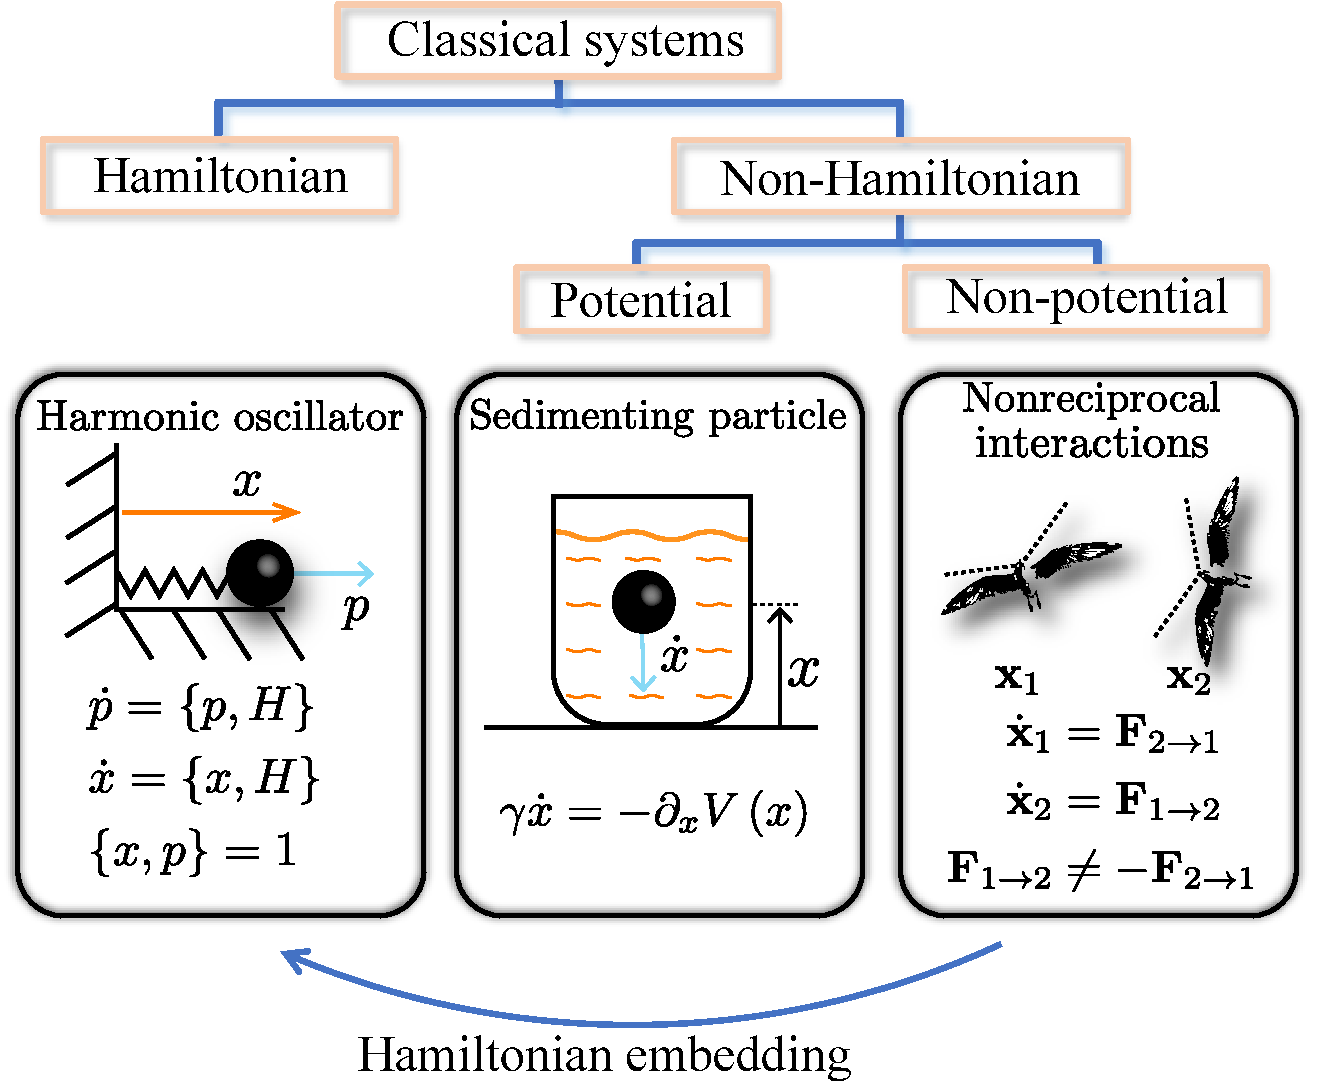
\includegraphics[width=0.5\textwidth]{./fig-01/my_fig.pdf}
	\caption{
		\textbf{One-sentence fig description.}
		Don't forget take-home message!
		List simulation parameters last. 
	}  
	\label{fig:intro}
\end{figure}

\section{Discussion and Outlook}

\textit{Acknolwdgements.---}%
...

\textit{Data availability statement.---}%
The data and code associated with this manuscript are available under [give explicit zenodo doi + cite reference].

\begin{appendix}

\section{My appendix}

\section{My appendix 2}

\end{appendix}

\else % no main text if mainmode=false
\fi % closes \ifmainmode

% ─── Supplementary Material ──────────────────────────────────────────────────────────────
\resumetoc
\ifsuppmode

\cleardoublepage



% re-define section and fig labels
\renewcommand{\thefigure}{S\arabic{figure}}
\setcounter{figure}{0}
\renewcommand{\theequation}{S.\arabic{equation}}
\setcounter{equation}{0}
\renewcommand{\thesection}{S\arabic{section}}
\setcounter{section}{0}


\onecolumngrid
\begin{center}
	\textbf{\large{\textit{\nqdcolor{Supplemental Material}}}}\\
	\hfill \break
\end{center}
\twocolumngrid

\ifcombinedmode
% don't show title and author names
\else
% print second author block
\maketitle
\fi % closes \ifcombinedmode

\tableofcontents

\section{Supplementary Sec}

\begin{figure*}[t!]
	\centering
	\includegraphics[width=1\textwidth]{./fig-S01/SI-fig.pdf}
	\caption{
		\textbf{One-sentence fig description.}
		Don't forget take-home message!
		List simulation parameters last. 
	}  
	\label{fig:SI}
\end{figure*}


\section{Supplementary Sec}


\subsection{Supplementary SubSec}



Supplemental lorem ipsum~\cite{dadhichi2020nonmutual}


\fi % closes \ifsuppmode

% ─── Bibliography ────────────────────────────────────────────────────────────
\bibliography{references}
	
\end{document}
